%%=============================================================================
%% Methodologie
%%=============================================================================

\chapter{\IfLanguageName{dutch}{Methodologie}{Methodology}}%
\label{ch:methodologie}

%% TODO: In dit hoofstuk geef je een korte toelichting over hoe je te werk bent
%% gegaan. Verdeel je onderzoek in grote fasen, en licht in elke fase toe wat
%% de doelstelling was, welke deliverables daar uit gekomen zijn, en welke
%% onderzoeksmethoden je daarbij toegepast hebt. Verantwoord waarom je
%% op deze manier te werk gegaan bent.
%% 
%% Voorbeelden van zulke fasen zijn: literatuurstudie, opstellen van een
%% requirements-analyse, opstellen long-list (bij vergelijkende studie),
%% selectie van geschikte tools (bij vergelijkende studie, "short-list"),
%% opzetten testopstelling/PoC, uitvoeren testen en verzamelen
%% van resultaten, analyse van resultaten, ...
%%
%% !!!!! LET OP !!!!!
%%
%% Het is uitdrukkelijk NIET de bedoeling dat je het grootste deel van de corpus
%% van je bachelorproef in dit hoofstuk verwerkt! Dit hoofdstuk is eerder een
%% kort overzicht van je plan van aanpak.
%%
%% Maak voor elke fase (behalve het literatuuronderzoek) een NIEUW HOOFDSTUK aan
%% en geef het een gepaste titel.
\begin{figure}[h]
    \centering
    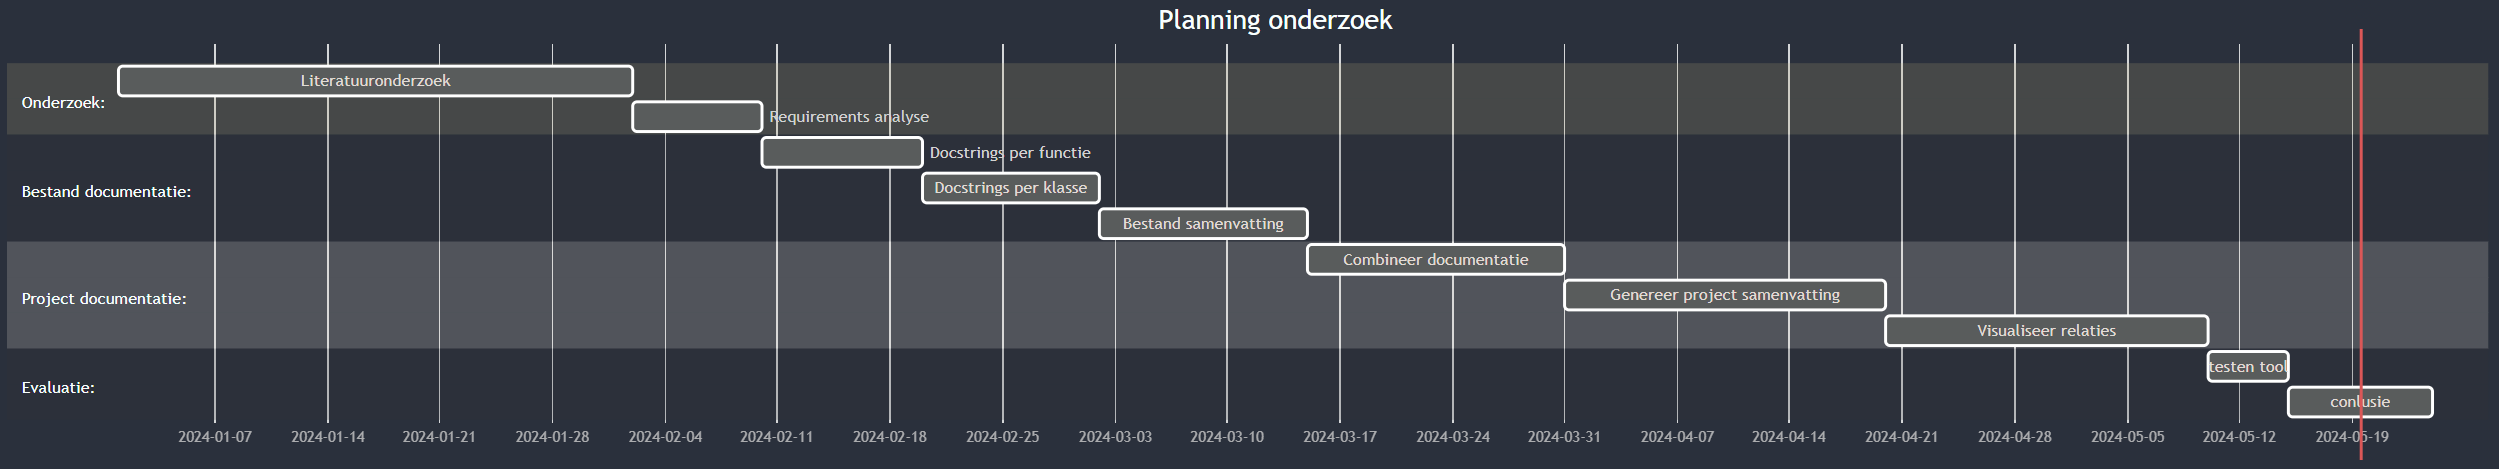
\includegraphics[width=1\textwidth]{flowchart.png}
    \caption{Tijdslijn onderzoek}
    \label{fig:flowchart}
\end{figure}

Het onderzoek is in drie fases opgedeeld. De eerste fase omvat de literatuurstudie.
In deze literatuurstudie wordt er onderzocht wat de huidige stand van zaken is omtent de technologie en mogelijkheden voor de documentatie van Python projecten met behulp van Large Language Modellen.
Zo wordt er gekeken naar wat LLM's zijn, hoe ze werken en wat bestaande tools zijn voor het genereren van documentatie.

Nadat er een duidelijk beeld gevormd is over de stand van zaken, kan er begonnen worden aan de tweede fase.
Hierin wordt er een tool ontwikkeld die een Python bestand kan analyseren op basis van de ongedocumenteerde code van het bestand.
Dit doet het eerst per functie dan per klasse en uiteindelijk voor het gehele bestand. Dit kan later gebruikt worden om een samenvatting van het project te genereren in de volgende fase.
De uitkomst van deze fase is een tool die de documentatie van een Python bestand kan genereren. 
Door aan prompt engineering te doen, met het prompt dat meegegeven wordt aan de LLM, kunnen de bekomen docstrings accurater worden.
Verder wordt er gekeken naar hoe de documentatie van Python functies gebruikt kan worden voor het maken van een gehele samenvatting van het project.
Dit wordt gedaan op basis van huidige methoden om docstrings aan te maken en te gebruiken. 
Erna kunnen de verschillende docstrings met de bijhorende naam van de functie of klasse gebruikt worden om een samenvatting te genereren.
Deze informatie kan dan gegeven worden aan de Large Language Modellen om een samenvatting te genereren.

De derde fase beslaagt het documenteren van een geheel project.
Door de vorige fases te combineren, het documenteren van de individuele bestanden en het genereren van een samenvatting van het project, kan er een tool gemaakt worden die de documentatie van een geheel project kan genereren.
Deze documentatie bestaat uit de individuele documentatie van de bestanden en een samenvatting van het gehele project. 
Alsook wordt er gekeken naar hoe de relaties tussen de verschillende bestanden gevisualiseerd kunnen worden.

De laatste fase is het evalueren van de tool.
Hier wordt er gekeken naar de kwaliteit van de documentatie die de tool genereert.
Dit wordt gedaan door de documentatie van de tool te vergelijken met de handgeschreven documentatie van een project.
Dit wordt gedaan voor een bestand, een klein project en een groot project.

\section{Requirementsanalyse}
\label{sec:requirements-analyse}
De requirementsanalyse is een belangrijk onderdeel van het onderzoek. 
Hier wordt er gekeken naar wat de tool moet kunnen en wat de verwachtingen zijn van de tool.

\subsection{Functionele requirements}
\label{sec:functionele-requirements}
\subsubsection{Should Have:}
\begin{itemize}
    \item De tool moet in staat zijn om docstrings te genereren voor functies en klassen voor een Python bestand.\\
    De tool genereert docstrings voor functies en klassen in een Python bestand. Dit gebeurt door de code te analyseren en op basis daarvan een docstring te genereren.
    \item De tool moet in staat zijn om een samenvatting van een Python bestand te genereren.\\
    De tool maakt een samenvatting van een Python bestand. In deze samenvatting zitten de belangrijkste zaken van het bestand.
    Zijnde de functies en klassen die erin voorkomen en wat deze doen, alsook hun eventuele parameters en de uitkomst.
    \item De tool moet in staat zijn om een samenhangende samenvatting van een Python project te genereren.\\
    De tool dient een samenvatting te maken van een Python project. Deze samenvatting bestaat uit de individuele samenvattingen van de bestanden en een overkoepelende samenvatting van het project.
    Hierin staan alle functies en klassen die in het project voorkomen en wat deze doen, alsook hun eventuele parameters en de uitkomst.
    \item De tool moet in staat zijn om de relaties tussen de verschillende bestanden van een project te visualiseren.\\
    De tool visualiseert  de relaties tussen de verschillende bestanden van een project. Zo is er geweten waar de bestanden naar verwijzen.
\end{itemize}

\subsubsection{Could Have:}
\begin{itemize}
    \item De tool moet in staat zijn om de documentatie van een Python bestand te genereren in verschillende formaten.\\
    De tool genereert de documentatie van een Python bestand in verschillende formaten. Zo kan de gebruiker kiezen in welk formaat de documentatie gegenereerd moet worden.
    \item De tool moet in staat zijn om de relaties tussen de verschillende functies en klassen van een bestand te visualiseren op project niveau.\\
    De tool visualiseert de relaties tussen de verschillende functies en klassen van een bestand op project niveau. Zo is er geweten welke functies en klassen gebruikt worden door de bestanden.
\end{itemize}

\subsubsection{Nice to Have:}
\begin{itemize}
    \item De tool moet in staat zijn om de documentatie van een Python bestand te genereren in verschillende talen.\\
    Zo kan de gebruiker kiezen in welke taal het bestand wordt gedocumenteerd.
\end{itemize}

\subsection{Niet-functionele requirements}
\label{sec:niet-functionele-requirements}
\subsubsection{Should Have:}
\begin{itemize}
    \item De tool moet betaalbaar zijn.\\
    Dit wil zeggen dat de tool geen hoge kosten met zich meebrengt.
    \item De tool moet leesbare documentatie genereren.\\
    De documentatie die de tool genereert moet leesbaar zijn. Dit wil zeggen dat de documentatie duidelijk moet zijn en dat de gebruiker er gemakkelijk informatie uit kan halen.    
\end{itemize}

\subsubsection{Nice to Have:}
\begin{itemize}
    \item De tool moet gebruiksvriendelijk zijn.\\
    Dit betekent dat de tool intuïtief moet zijn.
    \item De tool moet snel werken.\\
    Dit betekent dat de tool sneller documentatie moet genereren dan dat een persoon dit kan doen
\end{itemize}

\begin{table}
    \resizebox{\textwidth}{!}{
    \begin{tabular}{|l|l|l|l|l|l|}
    \hline
    Requirement & Should have & Could have & Nice to have & Functioneel & Niet Functioneel \\
    \hline
    Docstrings genereren voor functies en klassen & X & & & X & \\
    Samenvatting van een Python bestand genereren & X & & & X & \\
    Samenvatting van een Python project genereren & X & & & X & \\
    Relaties tussen verschillende bestanden visualiseren & X & & & X & \\
    Documentatie genereren in verschillende formaten & & X & & X & \\
    Relaties tussen verschillende functies en klassen visualiseren op project niveau & & X & & X & \\
    Documentatie genereren in verschillende talen & & & X & X & \\
    Betaalbaar & X & & & & X \\
    Leesbare documentatie genereren & X & & & & X \\
    Gebruiksvriendelijk & & & X & & X \\
    Snel werken & & & X & & X \\
    \hline
    \end{tabular}}
    \caption{Requirementsanalyse}
\end{table}

\section{Opstellen van een short-list tools}
\label{sec:long-list}
De short-list bestaat uit de verschillende tools die gebruikt kunnen worden voor het genereren van documentatie voor Pythonprojecten.
Deze tools worden onderzocht om te kijken welke het beste past bij de requirements van de tool die ontwikkeld wordt in dit onderzoek.

De oplijsting van de tools is gebaseerd op de literatuurstudie en bestaat uit de twee volgende tools:
\begin{itemize} 
\item GPT4Docstrings \autocite{Trofficus2023}\\
Een tool die docstrings genereert voor Python projecten met behulp van GPT4 \textcite{OpenAI2023}.
\item Doxygen \autocite{Doxygen2023}\\
Een tool die gebruikt wordt voor het genereren van documentatie voor projecten met reeds een docstring.
\end{itemize}

Deze tools worden verder onderzocht in de volgende hoofdstukken, GPT4Docstrings in het hoofdstuk \ref{sec:bestanddocumentatie-tool} en Doxygen in het hoofdstuk \ref{sec:project-documentatie-relaties}.